
\section{Shark Example}

\subsection{Query Execution Example}

Consider a Twitter-like application where users can broadcast short status messages and each user has certain profile information \eg age, gender, and location. The status messages themselves are kept in a \emph{messages} table along with a unique user identifier. Due to the volume of messages, they are partitioned by date. A \emph{profiles} table contains user information including country, gender, and age for each user id. 

{\small
\begin{verbatim}
CREATE TABLE messages (user_id INT, message STRING) 
    PARTITIONED BY (ds STRING);
CREATE TABLE profiles (user_id INT, country STRING, age INT);

LOAD DATA LOCAL INPATH '/data/messages'
INTO TABLE messages PARTITION (ds='2011-12-07');
LOAD DATA LOCAL INPATH '/data/profiles' INTO TABLE profiles;
\end{verbatim}
}

Suppose we would like to generate a summary of the top ten countries whose user have added the most status messages on Dec. 7, 2011. Furthermore, we would like to sort these results by number of messages in descending order. We could execute the following query:

{\small
\begin{verbatim}
FROM (SELECT * FROM messages a 
    JOIN profiles b ON 
    (a.user_id = b.user_id and a.ds='2011-12-07')
        ) q1
SELECT q1.country, COUNT(1) c 
    GROUP BY q1.country ORDER BY c DESC LIMIT 10
\end{verbatim}
}

The query contains a single join followed by an aggregation. Figure \ref{fig:hiveqp} is the query plan generated by Hive showing its map and reduce stages. Figure \ref{fig:sharkqp} shows the query plan as it is processed by Shark. For this query, Hive generates a three-stage map and reduce query plan. Note that the intermediate results after each MapReduce stage are written to HDFS in a temporary file in the FileSink operators. Since Spark and the RDD abstraction do not constrain us to the MapReduce paradigm, Shark can avoid this extra I/O overhead by simply writing intermediate results to local disk. Shark simply creates a new RDDs for each operator, reflecting an operator's transformation on the RDD that resulted from the previous operator's transformation. Any leaf operator is a table scan that generates an RDD from an HDFS file. 

Suppose that no previous queries have been run on this data or at least none have similar operator subtrees to the current query. At each operator stage where an RDD is substantially transformed, Shark adds the resulting RDD to the cache if caching for the given operator has not been disabled in the Shark configuration file.

\begin{figure}
	\centering
	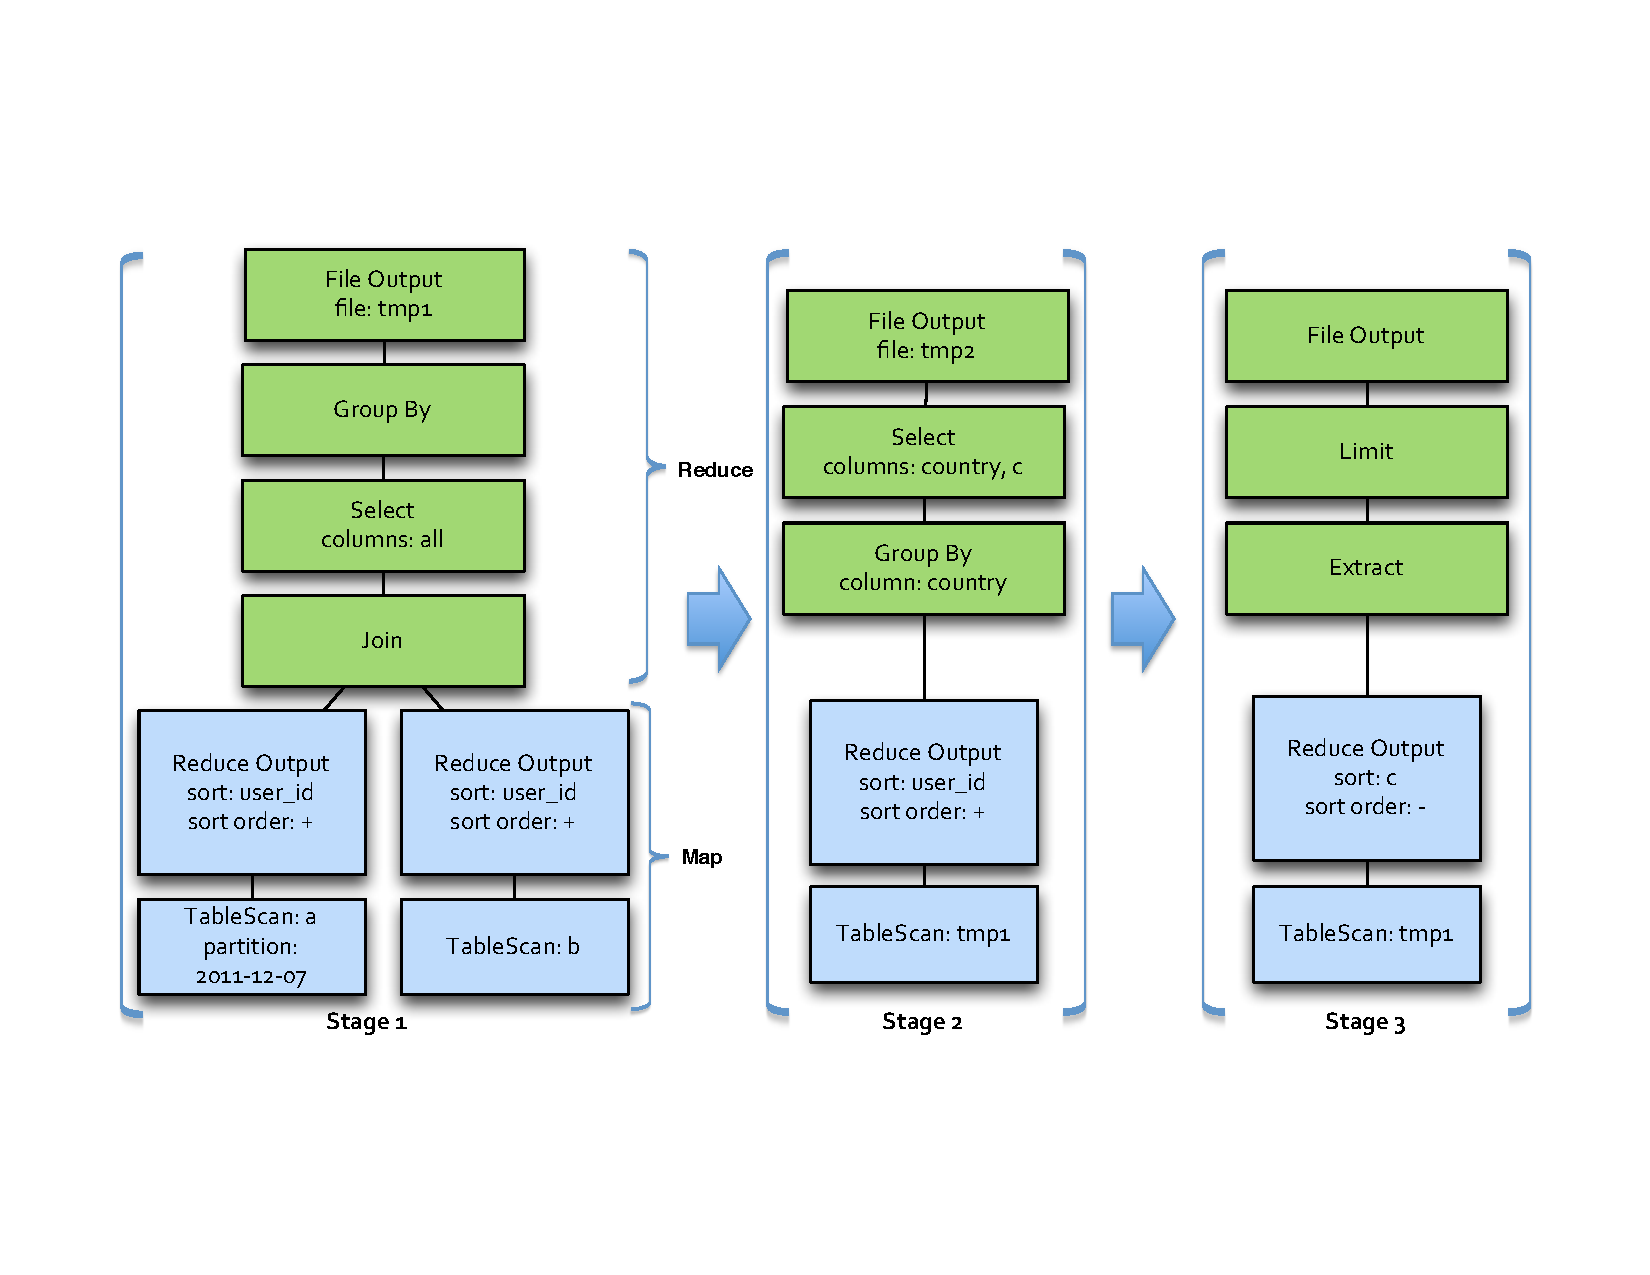
\includegraphics[width=\linewidth]{files/hive-qplan.pdf}
	\caption{Hive query plan}
	\label{fig:hiveqp}
\end{figure}

\begin{figure}
	\centering
	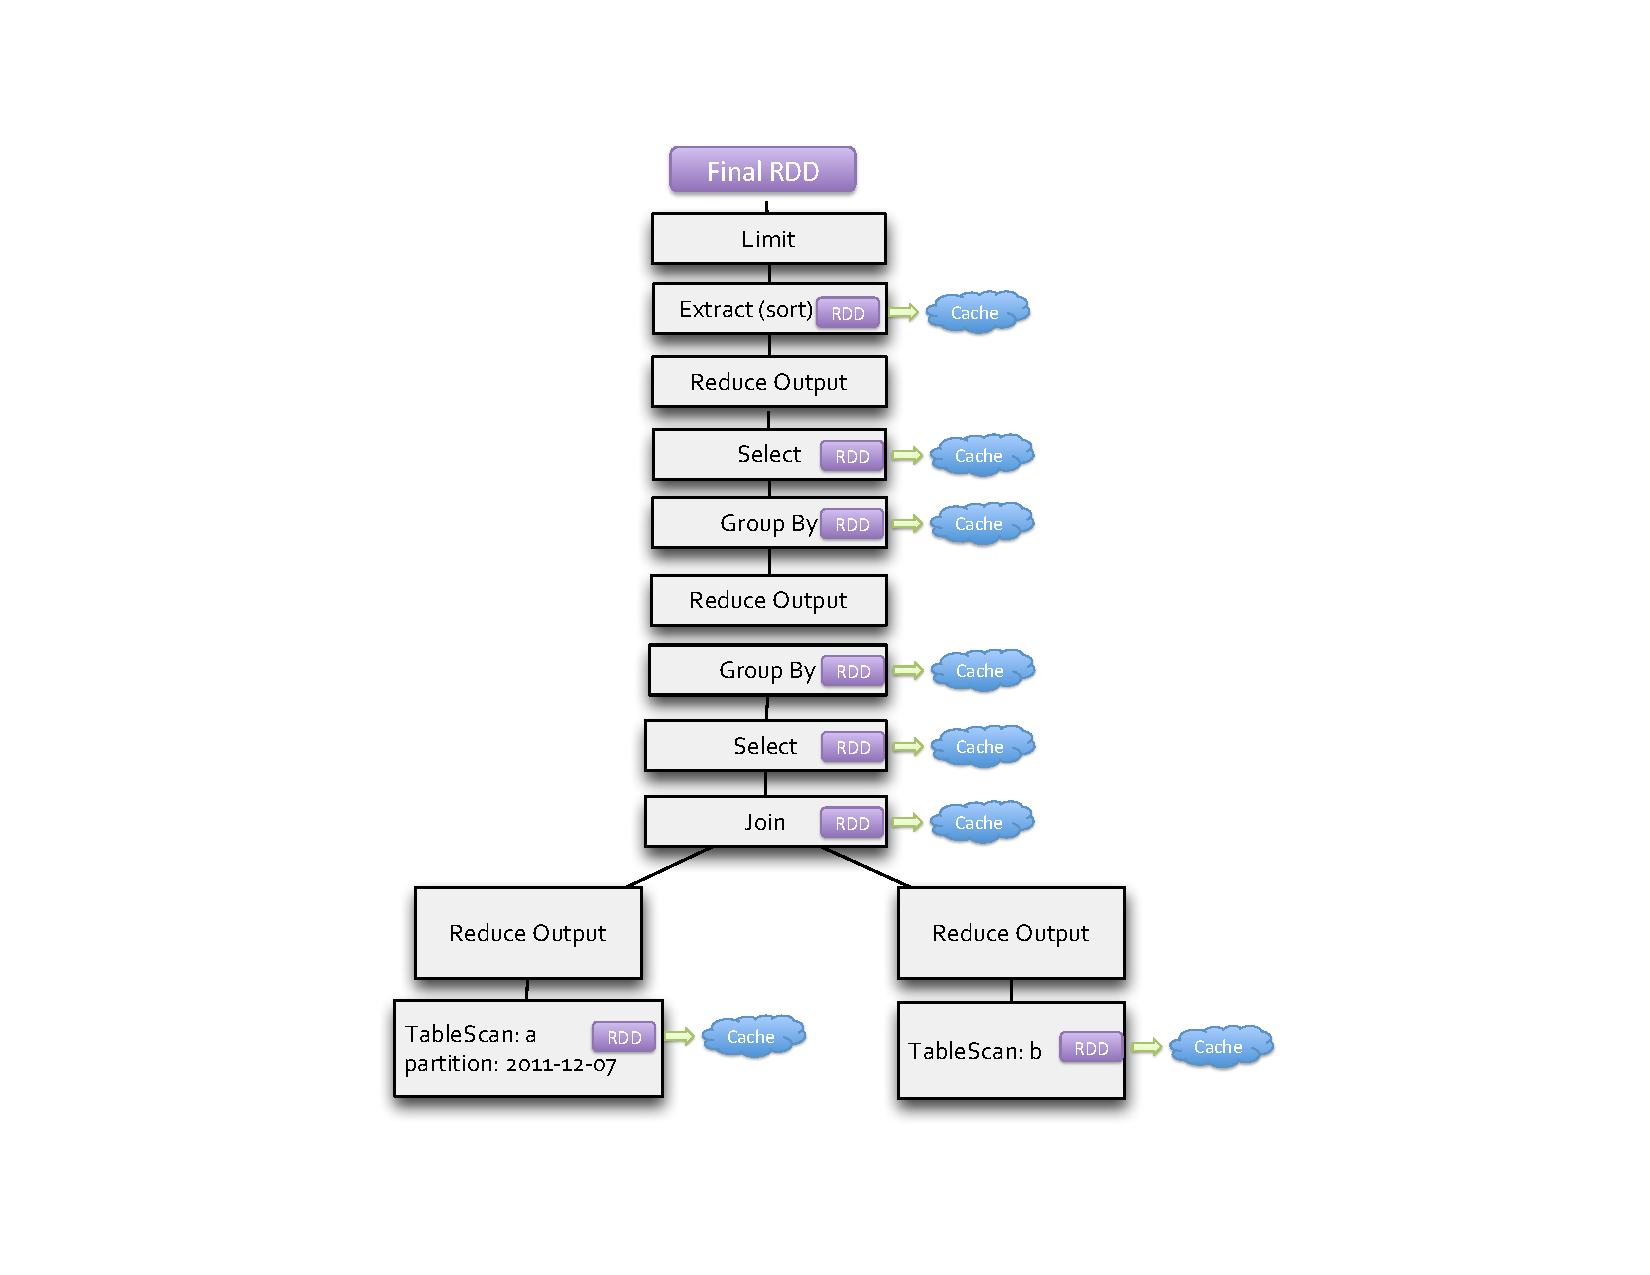
\includegraphics[width=\linewidth]{files/shark-qplan1.pdf}
	\caption{Shark query plan}
	\label{fig:sharkqp}
\end{figure}

Now, suppose that we would now like to query the same data to find the number of messages grouped by age instead. We could execute the following query. 

{\small
\begin{verbatim}
FROM (SELECT * FROM messages a 
    JOIN profiles b ON 
    (a.user_id = b.user_id and a.ds='2011-12-07')
        ) q1
SELECT q1.age, COUNT(1) c 
    GROUP BY q1.age ORDER BY age
\end{verbatim}
}

Apart from the omission of reading and writing intermediate data to HDFS, Shark's query plan is essentially identical up through the join by operator, so instead of generating new RDDs for each operation, existing RDDs for these operators will be found in memory. This is illustrated in Figure \ref{fig:sharkqp2}. The subsequent filter, group by, and order by operations require new transformations, and their resulting RDDs are stored in memory for future queries to use.

\begin{figure}
	\centering
	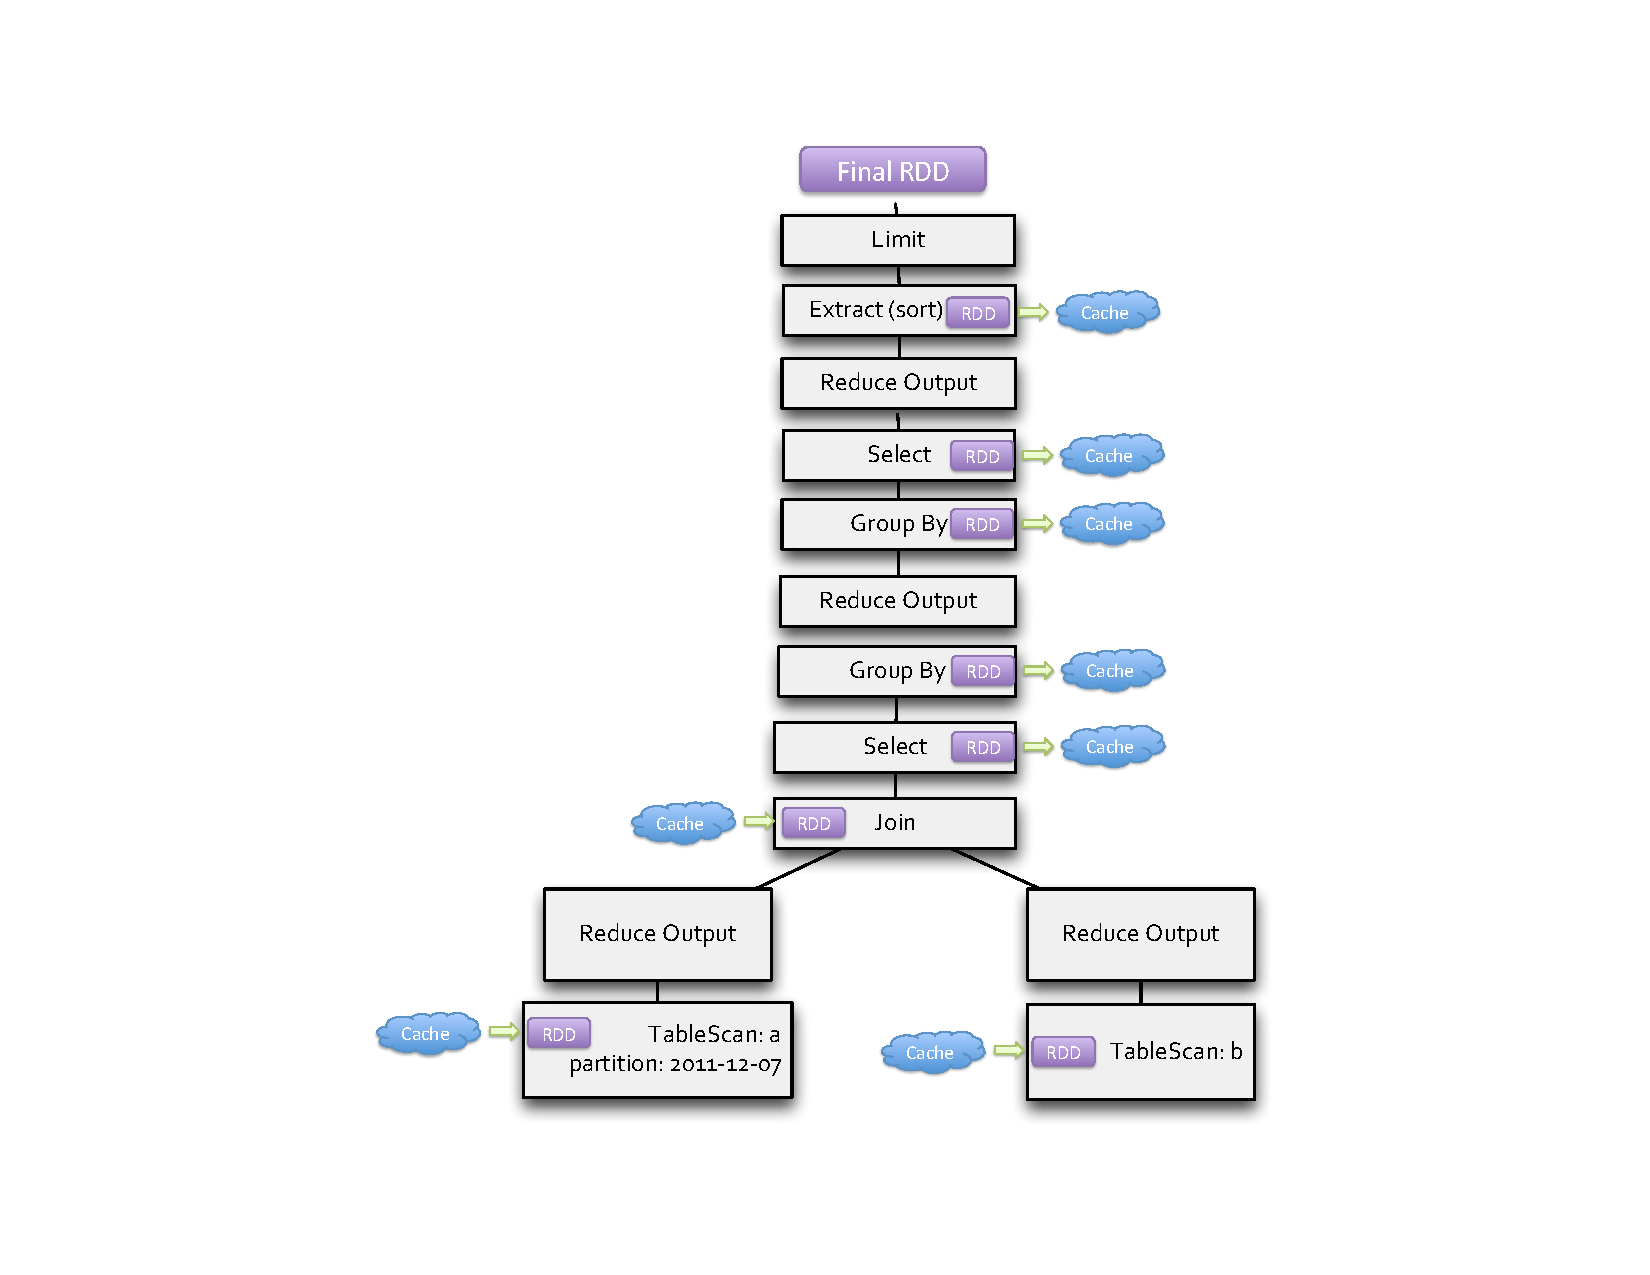
\includegraphics[width=\linewidth]{files/shark-qplan2.pdf}
	\caption{Shark query plan}
	\label{fig:sharkqp2}
\end{figure}


